V předchozí kapitole jsme si pověděli o analýze požadavků na systém.
Určili jsme si, kdo je uživatelem naší aplikace, co od naší aplikace očekává.
V tomto bodě jsme schopni teoreticky navrhnout architekturu našeho systému a přesně popsat požadovanou funkcionalitu, jakou budou disponovat jeho jednotlivé části.
Tato sekce se bude zabývat detailnějším rozborem konkrétních požadavků a návrhem architektury systému Coopmaster.

\clearpage
\section{Služby dle jednotlivých potřeb uživatele}\label{sec:microservices}
Jako teoretický model na základě kterého budeme organizovat a třídit funkcionalitu, jsem zvolil mikroservisní architekturu (sekce~\ref{sec:microservice-architecture}).
Tento způsob rozvržení zodpovědnosti částí systému jsem zvolil díky velké možnosti rozšíření, zapouzdření funkcionality a snadné úpravě jednotlivých služeb bez nutnosti kompletního restartu systému v případě znovunasazení.\newline
Jako programovací jazyk pro tvorbu služeb je zvolen programovací jazyk Python (sekce~\ref{sec:python}).
Python byl vybrán kvůli jeho univerzálnosti, snadné syntaxi a podpoře ze strany vývojářů a komunity.\newline
Pro realizaci, konfiguraci a síťování mikroservisní architektury je použit Docker Engine společně s rozšířením Docker Compose.\newline
Na základě předchozích rozhodnutí jsem tedy systém rozdělil do jednotlivých mikroslužeb tak, aby vznikla robustní a rozšiřitelná mikroservisní architektura a byly splněny všechny uživatelské požadavky, které jsme si určili (\ref{ch:tvorba-zadani}).\newline
Bylo tedy navrženo 8 služeb, které obsahují námi naprogramovanou funkcionalitu a dohromady společně s hardwarovými prvky tvoří systém Coopmaster.
\begin{itemize}
    \item Camera Driver (\ref{sec:camera-driver})
    \item Scale Driver (\ref{sec:scale-driver})
    \item Room Driver (\ref{sec:room-driver})
    \item Health Checker (\ref{sec:health-checker})
    \item Room Assistant (\ref{sec:room-assistant})
    \item Nest Watcher (\ref{sec:nest-watcher})
    \item Dog Alarm (\ref{sec:dog-alarm})
    \item Chicken Watch Guard (\ref{sec:chicken-watch-guard})
\end{itemize}

\clearpage
\section{Systém pro uživatelské rozhraní a automatizaci}\label{sec:systemu-pro-uzivatelske-rozhrani-a-automatizaci}
Podstatnou otázkou bylo, zda se pouštět do tvorby kompletně vlastního systému pro uživatelské rozhraní a automatizaci.
Po zvážení časové náročnosti, technologické náročnosti a komplexnosti takového systému, mi bylo jasné, že tudy cesta nepovede.
Bylo tedy třeba najít open source systém, který již touto funkcionalitou disponuje.
Nakonec jsem zvolil systém Home Assistant, protože jsem s ním již dříve pracoval a mám s ním dobré zkušenosti~\cite{homeassistant-web}.
Home Assistant má na internetu také rozsáhlou podporu.
Má bohaté diskuzní forum a širokou komunitu.
Zároveň je možné nahlédnout do již hotových řešeních pro inspiraci.
Jak je nakonfigurováno uživatelské rozhraní v Home Assistantovi, je popsáno v části~\ref{sec:tvorba-gui-rozhrani}.

\clearpage
\section{Komunikace mezi moduly}\label{sec:komunikace-mezi-backendem-a-frontendem}
Je třeba zajistit komunikaci mezi systémem Home Assistant a Coopmaster službami.
Tuto úlohu musíme přijmout velice zodpovědně a navrhnout řešení, které půjde opět snadno rozšířit a modifikovat.
Z toho důvodu nelze použít klasický \gls{http}, protože bychom komunikaci vázali na doménové jméno a port nebo ip adresu a port.
Toto řešení má problém v tom, že pokud bychom potřebovali změnit, buď umístění částí služeb nebo port jedné ze služeb, bylo by třeba překonfigurovat i Home Assistanta.
Další problém nastane, když potřebujeme z některé ze služeb poslat například notifikaci do Home Assistanta, je pro to potřeba, aby jednotlivé služby věděly, kde na síti Home Assistant běží, což je věc, která se může měnit, a museli bychom naopak přenastavovat jednotlivé služby.
Jako řešení se nabízí použít messaging konkrétně třeba technologii \gls{mqtt} (část~\ref{sec:mqtt}).
Tato technologie se běžně používá u \gls{iot} zařízení a pro naše použití je vynikajícím řešením.

\clearpage
\section{Hardwarová zařízení}\label{sec:hardwarova-zarizeni}
Tuto sekci je velmi důležité dobře a správně navrhnout, protože náš systém bude pracovat s daty z reálného světa.
Tato data musejí získávat k tomu určená zařízení a na jejich přesnosti závisí efektivita a správnost chování zbytku systému.
Musíme tedy navrhnout a realizovat několik zařízení, která společně budou plnit následující úlohy
\begin{itemize}
    \item Snímání stavů hnízd
    \item Ovládání dvířek
    \item Snímání teploty
    \item Snímání vlhkosti
    \item Snímání interiéru kurníku
    \item Snímání výběhu
\end{itemize}

\subsection{Snímání stavů hnízd}
Všechny případy, které potřebujeme řešit v kontextu našeho hnízda, se dají rozpoznat na základě hmotnosti hnízda.
Pokud je v hnízdě slepice, hnízdo bude hodně zatížené oproti počátečnímu prázdnému stavu.
V případě, že bude hnízdo zatížené málo a nebo středně, může to pro nás ve většině případů spolehlivě znamenat, že se v hnízdě nacházejí vejce.
Nestandardní situace jako neobvyklý nepořádek v hnízdě, případně výkal, řešit nebudeme, protože by to exponenciálně zvýšilo složitost řešení a nepřineslo by to o moc lepší data.
Kurník ja navíc v našem případě pravidelně udržován, takže šance na výskyt chybového faktoru v podobě nežádoucí zátěže je nízká.
Jako nejjednodušší prostředek pro splnění tohoto úkolu na základě předchozí analýzy se ukázala obyčejná digitální váha.
Bude třeba vytvořit vlastní konstrukci vzhledem ke skutečnosti, že ji musíme zabudovat do již existujícího hnízda.
Popis konkrétního zapojení a konstrukce je sepsán níže v sekci~\ref{sec:digitalni-vaha-do-hnizda}.

\subsection{Ovládání dvířek, snímání teploty a vlhkosti}
Pro ovládání dvířek a snímání povětrnostních podmínek je nejrozumnější vytvořit řídící jednotku, která tyto požadavky obsáhne.
Další částí jsou samotná elektrická dvířka. Na základě elektrického signálu budou otevřená nebo zavřená.
Teplota a vlhkost jsou snímány senzory, jež jsou součástí řídící jednotky.
Řídící jednotka je popsána v sekci~\ref{sec:ridici-jednotka} a konstrukce dvířek v sekci~\ref{sec:konstrukce-dvirek}.

\subsection{Snímání scén v kurníku a ve výběhu}
Ke snímání scén v daných oblastech je třeba vybrat zařízení s dostatečnou odolností proti povětrnostním vlivům.
Speciálně v kurníku je hodně agresivní prostředí kvůli vysoké vlhkosti.
Pro dlouhodobý provoz je třeba vybrat kvalitní a odolnou techniku.
Zařízení musí být připojeno přes Ethernet a musí být napájené ze sítě, nikoli pomocí baterie.
Pro vývoj a testování jsem používal klasickou webovou kameru, ale pro produkční nasazení jsem na základě předešlé analýzy rozhodl o použít venkovní IP kameru.
Kamera musím mít následující vlastnosti
\begin{itemize}
    \item Dostatečná odolnost proti vniknutí cizího tělesa a kapalin
    \item Dobrou kvalitou obrazu
    \item Velké zorné pole
    \item Jednoduchou instalaci
    \item Cenová dostupnost
    \item Kvalitní signál pro potřeby rozpoznávání
\end{itemize}
Podrobnosti ohledně výběru kamery se nachází v části~\ref{sec:kamerovy-system}

\clearpage
\section{Spolupráce modulů dle požadavků uživatele}\label{sec:schematicka-vyjadreni-zavislosti-jednotlivych-modulu}

\subsection{Ovládání světla, data o teplotě a vlhkosti}
Každý tvor potřebuje k životu světlo a teplo a ani u slepiček to není jinak.
Prodlužováním dne se jim prodlužuje čas, kdy se krmí a jsou aktivní.
Zajištěný tepelný komfort přispívá jejich pohodě a následně větší produkci vajec.
Tato část je tedy důležitá pro chovatele, aby měl na dálku přehled o podmínkách v kurníku, a to převážně o teplotě.
Dalším z požadavkům bylo dálkové ovládání a automatizace světla, čehož se tato sekce také dotýká.
Graficky jsou použité moduly a jejich závislosti vyjádřeny v obrázku~\ref{fig:svetlo_teplo_vlhkost}.\newline

\begin{figure}[H]
    \centering
    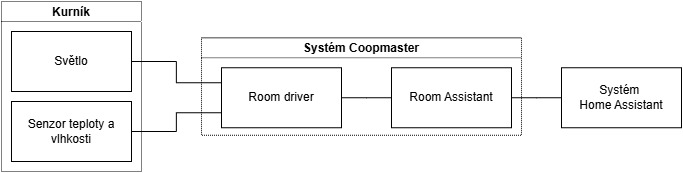
\includegraphics[width=0.8\textwidth]{img/svetlo_teplo_vlhkost}
    \captionAuthorSource{Diagram komunikace mezi relé a sonzory}
    \label{fig:svetlo_teplo_vlhkost}
\end{figure}

Hardwarový prvek, který dokáže ovládat světlo a zpřístupňuje systému informace o teplotě a vlhkosti, je řídící jednotka.
Ta je přes USB sběrnici propojena s Room Driverem, který je již součástí Docker Composu Coopmasteru.
Room Driver je použit jako mezičlen pro komunikaci mezi hardwarovými prvky a výkonným kódem.
Výkonný kód se nachází ve službě Room Assistant.
Room Assistant je s Room Driverem propojen pomocí HTTP protokolu a dále komunikuje se systémem Home Assistant díky messaging protokolu MQTT.
Home Assistant v této sekci poskytuje uživateli data o teplotě, vlhkosti a stavu světla.
Uživatel pak může za pomoci Home Assistanta vysílat požadavky na změnu stavu světla.
Data o teplotě a vlhkosti Room Assistant aktualizuje každých 10 vteřin.


\subsection{Automatizace dvířek}
Jeden z klíčových požadavků, díky kterým vznikl tento projekt, je zautomatizování ranního otevírání a večerního zavírání dvířek v kurníku.
V této části si tedy zjednodušeně popíšeme princip, jak je v systému Coopmaster řešené automatické ovládání dvířek.
Graficky jsou závislosti mezi jednotlivými moduly vysvětleny v obrázku~\ref{fig:automatizace_dvirek}.\newline
Dvířka v našem systému jsou kontrolována pomocí modulu řídící jednotka.
Module Room Driver zajišťuje pomocí USB sběrnice a HTTP protokolu komunikaci mezi řídící jednotkou a Room Assistantem.
Room Assistant je propojen se systémem Home Assistant pomocí MQTT protokolu.
Dále potřebuji získat data z kamerového systému konkrétně z kamery v kurníku.
Komunikaci s kamerovým systémem zajišťuje přes HTTP protokol modul Camera Driver.
Tento modul má vystavené \gls{rest} \gls{api} a poskytuje obrázky službám v systému Coopmaster.
O obrázky si zde říká služba Chicken Watch Guard, která za pomocí neuronové sítě, konkrétně pak metody klasifikace~\cite{klasifikace}, počítá slepice v kurníku a výsledný počet posílá opět pomocí MQTT do Home Assistanta.
Chicken Watch Guard také předává co minutu do systému Home Assistant obrázek z kamery v kurníku.
Home Assistant tedy pro tuto komponentu zajišťuje indikaci stavu dvířek, ovládací tlačítka pro dvířka, vizualizaci počtu slepic v kurníku a zobrazuje fotografii pořízenou v kurníku.
Home Assistant je nakonfigurován tak, aby se od určitého časového okamžiku snažil zavřít dvířka pod podmínkou, že bude počet slepic, který identifikoval Chicken Watch Guard, stejný jako ten, jež jsme nastavili jako pevnou konstantu neboli aktuální počet slepic v kurníku.
\begin{figure}[H]
    \centering
    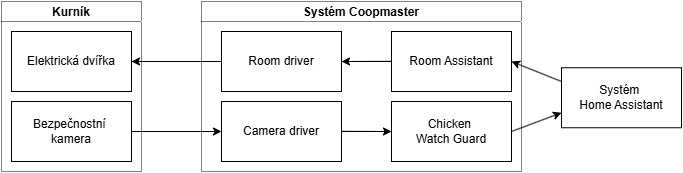
\includegraphics[width=0.8\textwidth]{img/automatizace_dvirek}
    \captionAuthorSource{Diagram bezpečného zavření dvířek}
    \label{fig:automatizace_dvirek}
\end{figure}

\subsection{Detekce vetřelců}
Pro tento úkol bude třeba využít obrázků z kamery ve výběhu a umělé inteligence, která v obraze rozpozná určené vetřelce.
Princip komunikace je graficky vysvětlen v obrázku~\ref{fig:detekce_vetrelcu}.\newline
S kamerou ve výběhu komunikuje pomocí HTTP protokolu služba Camera Driver.
Z REST aplikačního rozhraní služby si stahuje obrázky služba Dog Alert.
Tato služba využívá neuronovou síť~\cite{neuronovesite} k detekci vetřelce v obraze.
Pokud je detekováno nějaké nebezpečí, služba pomocí MQTT protokolu informuje systém Home Assistant a předá mu aktuální fotografii, v níž byl vetřelec detekován jako důkaz.
Home Assistant je nastaven tak, že při přijetí takové zprávy, odešle uživateli do aplikace v mobilním telefonu oznámení, aby ho upozornil na detekci hrozby.
Dog Alarm dále pak každou minutu posílá do Home Assistanta aktuální snímek z kamery ve výběhu, aby měl uživatel stále přehled.
\begin{figure}[H]
    \centering
    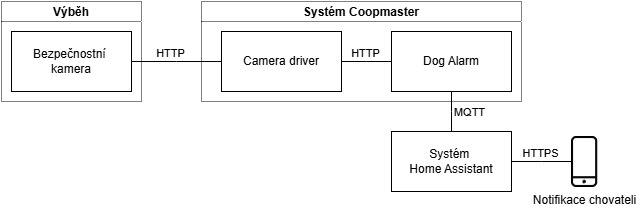
\includegraphics[width=0.8\textwidth]{img/detekce_vetrelcu}
    \captionAuthorSource{Diagram detekce vetřelců}
    \label{fig:detekce_vetrelcu}
\end{figure}

\subsection{Vizualizace stavů hnízd}
Abych mohl splnit tento požadavek, bude potřeba získat údaje o aktuální hmotnosti z jednotlivých vah ve hnízdech.
Tato data je pak nutné předat do služby Nest Watcher.
Nest Watcher následně data vyhodnotí a výsledky předá k vizualizaci do systému Home Assistant.
Schématické vyjádření principu pro vizualizaci stavů hnízd je znázorněno na obrázku~\ref{fig:vizualizace_stavu_hnizd}. \newline
Pro komunikaci s modulem digitální váhy je použita služba Scale Driver, která s jednotlivými váhami komunikuje přes USB sběrnici.
Data o váhách si ze Scale Driveru stahuje služba Nest Watcher.
Tato služba ukládá v daném intervalu data z každé váhy do databáze.
Služba po uplynutí časové konstanty analyzuje časovou řadu v databázi a vyhodnotí stav hnízda.
Detailní popis algoritmu je v části věnované službě Nest Watcher (\ref{sec:nest-watcher}).
Po vyhodnocení stavů jsou data předávána pomocí MQTT protokolu do systému Home Assistant, který je díky na míru dělané komponentě zobrazí uživateli.
\begin{figure}[H]
    \centering
    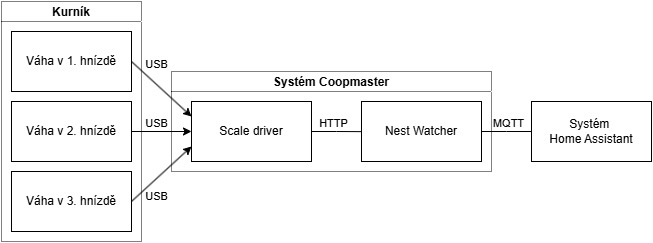
\includegraphics[width=0.8\textwidth]{img/vizualizace_stavu_hnizd}
    \captionAuthorSource{Diagram vizualizace stavů hnízd}
    \label{fig:vizualizace_stavu_hnizd}
\end{figure}

\clearpage
\section{Zpřístupnění aplikace z internetu}\label{sec:zpristupneni-aplikace-z-internetu}
Aby systém mohl sloužit svému účelu, musí být vzdáleně přístupný.
To znamená, že server, na kterém systém poběží, musí mít veřejnou \gls{ip} adresu a v ideálním případě mít tuto adresu propojenou s doménovým názvem pro snadnější použití.
Tato problematika se dá řešit několika způsoby.\newline
Jeden ze způsobů je zřízení veřejné IP adresy pro svůj server.
Toto řešení je, technicky i teoreticky náročné, protože v případě, se kterým pracujeme my, běží server na lokální síti a veřejná IP adresa tedy není přímo pro náš server, ale celou síť.
To vytváří v určitých situacích velmi vážná bezpečnostní rizika, díky čemuž je tato metoda velice náročná na hardware a implementaci.
Navíc poskytování veřejné IP adresy je placená služba poskytovatele internetového připojení.\newline
Další způsob je nasazení části systému do některého z cloudových řešení jako je Microsoft Azure~\cite{aml} nebo Amazon~\cite{AWS} \gls{aws}.
Tato metoda by v podstatě vyhovovala našim požadavkům, ale pokud bychom se bavili o ceně, tak to rozhodně není levné řešení. \newline
Metoda, kterou využíváme v našem řešení, je snadná, jednodušší na implementaci než zřizování veřejné IP adresy a levnější než využití cloudové služby.
Tento způsob využívá takzvané tunely neboli šifrovaná spojení.
Funguje na principu, při němž zařízení šifrovaně propojíte s veřejným serverem a tento server bude skrze sebe vystavovat službu, která běží na lokálním počítači například u nás doma.
Výhoda je, že vzdálený server disponuje kvalitním a odborně nastaveným firewalem, který zajistí dobrou ochranu našeho lokálního serveru.
Tuto službu poskytuje zdarma a bez omezení například společnost Cloudflare~\cite{cloudflare}.
Tento způsob nejvíce odpovídá našim požadavkům, kterými byly cena a jednoduchost, společně s rychlostí nasazení.
Pro lepší znázornění komunikace mezi moduly přikládám schéma ~\ref{fig:vizualizace_stavu_hnizd}.

\begin{figure}[H]
    \centering
    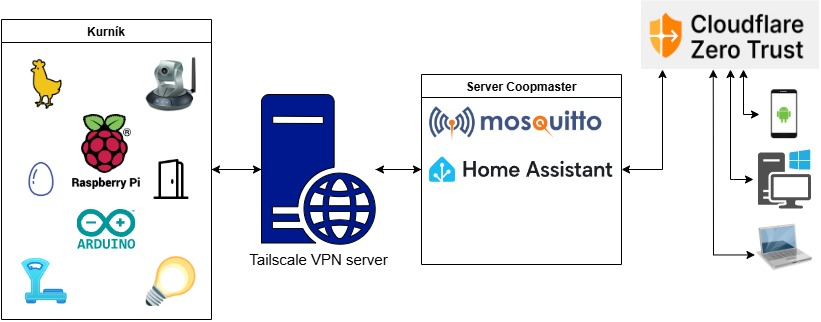
\includegraphics[width=\textwidth]{img/orientacni_topologie}
    \captionAuthorSource{Orientační topologie systému}
    \label{fig:orientacni_topologie}
\end{figure}

Poslední nutností, kterou ovšem je třeba zaplatit, je pronájem vlastního doménového jména.
Doménu si lze pronajmout u doménových registrátorů jako jsou GoDaddy~\cite{GoDaddy}, Hostinger~\cite{Hostinger} nebo například Forpsi~\cite{forpsi}.
Ceny domén se odvíjí na základě jejího druhu a pohybují od 20 do 1500 korun za kus.
My v našem řešení využíváme službu Forpsi, protože s ní mám již předchozí zkušenost.\newline
Dále je tato část rozvedena v sekci~\ref{ch:nasazeni-systemu-do-produkce}, kde je popsán konkrétní způsob nasazení do funkčního projektu.



